\chapter{Implementasi dan Pengujian Perangkat Lunak}
\label{chap:implementasidanpengujian}

Bab ini terdiri atas dua bagian, yaitu Implementasi Perangkat Lunak dan
Pengujian Perangkat Lunak. Bagian implementasi berisi penjelasan lingkungan
pengembangan perangkat lunak. Sedangkan bagian pengujian berisi hasil pengujian
terhadap perangkat lunak yang telah dibangun.

\section{Implementasi Perangkat Lunak}
\label{sec:implementasiperangkatlunak}

Pada bagian ini akan dibahas hasil implementasi perangkat lunak yang telah
dibangun. Subbab ini terdiri atas tiga bagian, yaitu lingkungan perangkat keras,
lingkungan perangkat lunak, dan hasil implementasi perangkat lunak.

\subsection{Lingkungan Implementasi Perangkat Keras}
\label{sec:lingkunganimplementasiperangkatkeras}

Dalam membangun perangkat lunak ini digunakan spesifikasi perangkat keras sebagai berikut:

\begin{enumerate}
\item[(a)] Processor: AMD A10-5750M 2.5GHz
\item[(b)] RAM: 4 GB DDR3
\item[(c)] Harddisk: 1TB
\item[(d)] VGA: AMD Radeon HD 8650G 2GB
\item[(e)] Koneksi Internet: WAN
\end{enumerate}

\subsection{Lingkungan Implementasi Perangkat Lunak}
\label{sec:lingkunganimplementasiperangkatlunak}

Dalam membangun perangkat lunak ini digunakan spesifikasi perangkat lunak sebagai berikut:

\begin{enumerate}
\item[(a)] Sistem Operasi: Windows 8.1 Pro 64-bit
\item[(b)] Bahasa Pemrograman: PHP Version 5.6.3
\item[(c)] Aplikasi: XAMPP v5.6.3
\item[(d)] Aplikasi web browser: Google Chrome
\item[(e)] Library: Google APIs Client Library untuk PHP
\item[(f)] Javascript: Strapdown.js
\item[(g)] Framework: Foundation
\end{enumerate}

\subsection{Hasil Implementasi Perangkat Lunak}
\label{sec:hasilimplementasi}

Kode program perangkat lunak ditulis berdasarkan perancangan yang telah dibahas
pada bab~\ref{chap:perancangan}. Kode program untuk membangun  menggunakan PHP
dengan library Google APIs Client.

\section{Pengujian Perangkat Lunak}
\label{sec:pengujianperangkatlunak}

Pada bagian ini akan dibahas mengenai pengujian yang akan dilakukan terhadap
perangkat lunak. Pengujian tersebut terdiri dari dua bagian yaitu pengujian
fungsional dan pengujian eksperimental. Pengujian fungsional bertujuan untuk
memastikan bahwa seluruh fungsi yang dibangun pada perangkat lunak berjalan
sesuai dengan yang direncanakan. Sedangkan pengujian eksperimental bertujuan
untuk menguji eksepsi-eksepsi yang terdapat pada perangkat lunak. Pada bagian
ini juga terdapat perubahan program pada bagian oauth.php, jadi dapat
menjalankan pengujian dengan email yang diakhiri @student.unpar.ac.id
dikarenakan penulis tidak memiliki email yang diakhiri @unpar.ac.id.

\subsection{Lingkungan Pengujian Perangkat Keras}
\label{sec:lingkunganpengujianperangkatkeras}

Dalam pengujian perangkat lunak ini digunakan spesifikasi perangkat keras sebagai berikut:

\begin{enumerate}
\item[(a)] Processor: AMD A10-5750M 2.5GHz
\item[(b)] RAM: 4 GB DDR3
\item[(c)] Harddisk: 1TB
\item[(d)] VGA: AMD Radeon HD 8650G 2GB
\item[(e)] Koneksi Internet: WAN
\end{enumerate}

\subsection{Lingkungan Pengujian Perangkat Lunak}
\label{sec:lingkunganpengujianperangkatlunak}

Dalam pengujian perangkat lunak ini digunakan spesifikasi perangkat lunak sebagai berikut:

\begin{enumerate}
\item[(a)] Sistem Operasi: Windows 8.1 Pro 64-bit
\item[(b)] Bahasa Pemrograman: PHP Version 5.6.3
\item[(c)] Aplikasi: XAMPP v5.6.3
\item[(d)] Aplikasi web browser: Google Chrome
\item[(e)] Library: Google APIs Client Library untuk PHP
\item[(f)] Javascript: Strapdown.js
\item[(g)] Framework: Foundation
\end{enumerate}

\subsection{Pengujian Fungsional}
\label{sec:pengujianfungsional}
Pengujian fungsional menguji tampilan antar muka perangkat lunak beserta fungsi
dasar. Berikut ini adalah daftar pengujian yang dilakukan:
\begin{enumerate}[(1)]
\item Fungsi login\\
	Pengujian fungsi ini dilakukan untuk memastikan perangkat lunak terhubung ke
	server google untuk melakukan otentikasi dan otorisasi serta memeriksa apakah
	email yang digunakan untuk login diakhiri "@unpar.ac.id" atau
	"@student.unpar.ac.id" dikarenakan penulis tidak mempunyai akun dosen. Contoh
	kasus adalah melakukan login sebanyak dua kali, yang pertama menggunakan email
	yang diakhiri "@unpar.ac.id" atau "@student.unpar.ac.id", dan yang kedua
	menggunakan email yang diakhiri selain "@unpar.ac.id" dan
	"@student.unpar.ac.id". Pengujian pertama pengguna membuka halaman index.php
	dapat dilihat pada Gambar \ref{fig:membukahalamanindex}. Lalu pengguna melakukan
	login menggunakan email "7310013@sudent.unpar.ac.id" dapat dilihat pada Gambar
	\ref{fig:logindenganstudent}. Lalu akan ada konfirmasi bahwa akun yang digunakan
	dikelola oleh student.unpar.ac.id dapat dilihat pada Gambar
	\ref{fig:konfirmasiemail}. Lalu pengguna akan diarahkan ke CAS (Central
	Authentication Service) UNPAR dan melakukan login kembali dapat dilihat pada
	Gambar \ref{fig:casunpar}. Lalu pengguna akan diminta untuk memberikan izin
	aksses dari pihak pengguna dapat dilihat pada Gambar
	\ref{fig:izindaripihakpengguna}. Setelah pengguna memberikan izin akses maka
	akan dilakukan dengan fungsi memilih mahasiswa yang akan dibahas pada poin
	berikutnya. Sedangkan pengujian kedua pengguna melakukan login menggunakan
	email "bletack@gmail.com" dapat dilihat pada Gambar \ref{fig:logindengangmail}.
	Lalu pengguna akan mendapat alert karena email yang digunakan tidak sesuai
	dengan ketentuan dapat dilihat pada Gambar \ref{fig:alert}. Setelah pengguna
	menekan tombol ok pada alert maka pengguna akan dikembalikan ke halaman
	index.php. Hal ini menunjukkan fungsi login sudah berjalan dengan baik.
\item Fungsi memilih mahasiswa\\
	Pengujian fungsi ini dilakukan untuk memastikan pengguna dapat memilih
	mahasiswa. Pada halaman list.php terdapat tabel yang berisikan npm, nama, dan
	last update dan pengguna dapat memilih mahasiswa dengan menekan npm yang
	diinginkan. Contoh pengujian pengguna akan memilih mahasiswa dengan npm
	2010730013 maka akan menghasilkan link yang mengarah ke
	$view.php?npm=2010730013$ dapat dilihat pada Gambar \ref{fig:memilihmahasiswa}.
	Hal ini menunjukkan fungsi memilih mahasiswa sudah berjalan dengan baik.
\item Fungsi melihat info mahasiswa\\
	Pengujian fungsi ini dilakukan untuk memastikan mahasiswa yang telah dipilih
	oleh pengguna, dapat dilihat info dari mahasiswa tersebut. Contoh pengujian
	fungsi merupakan lanjutan dari fungsi memilih mahasiswa, dimana setelah
	pengguna memilih mahasiswa pada list.php maka akan menampilkan info dari
	mahasiswa tersebut dapat dilihat pada Gambar \ref{fig:melihatinfomahasiswa}.
	Hal ini menunjukkan fungsi melihat info mahasiswa sudah berjalan dengan baik.
\item Fungsi mengedit info mahasiswa\\
	Pengujian fungsi ini dilakukan untuk memastikan info mahasiswa dapat diedit.
	Contoh pengujian mengambil info dari mahasiswa yang telah dilihat infonya pada
	fungsi melihat info mahasiswa. Dimana keterangan info mahasiswa yang ada akan
	ditampilkan dan pengguna dapat mengedit lalu menyimpan perubahan dengan menekan
	tombol "Simpan" dapat dilihat pada Gambar \ref{fig:mengeditinfomahasiswa}.
	Setelah menyimpan perubahan pengguna akan dibawa kembali ke halaman list.php.
	Hal ini menunjukkan fungsi mengedit info mahasiswa sudah berjalan dengan baik.
\item Fungsi melihat histori\\
	Pengujian fungsi ini dilakukan untuk memastikan adanya histori dari mahasiswa
	yang dipilih lalu dapat melihat versi keterangan yang pertama kali dibuat dan
	versi-versi berikutnya yang sudah dirubah. Contoh pengujian melihat histori
	dari mahasiswa dengan npm 2010730013 dapat dilihat pada Gambar
	\ref{fig:melihathistori} dan juga melihat keterangan versi pertama berserta
	versi berikutnya dapat dilihat pada Gambar \ref{fig:keteranganversipertama} dan
	Gambar \ref{fig:keteranganversikedua}. Hal ini menunjukkan fungsi melihat
	histori sudah berjalan dengan baik.
\item Fungsi membuat entri baru\\
	Pengujian fungsi ini dilakukan untuk memastikan pada saat membuat entri baru
	terdapat template markdown dan berhasil menyimpan entri baru tersebut. Contoh
	pengujian menambahkan entri baru dengan npm 2010730012, nama Kevin PL, dan
	keterangan sesuai template. Terdapat template markdown pada saat membuka
	halaman new.php dapat dilihat pada Gambar \ref{fig:templateentribaru}. Mengisi
	data npm 2010730012 dan nama Kevin PL dapat dilihat pada Gambar
	\ref{fig:membuatentribaru}. Setelah pengguna menekan tombol "Simpan" maka data
	yang telah dimasukan akan tersimpan dan pengguna akan dikembalikan ke halaman
	list.php. Pengguna dapat melihat entri baru dengan npm 2010730012 dan nama
	Kevin PL telah masuk kedalam tabel dapat dilihat pada Gambar
	\ref{fig:entribaruberhasil}. Hal ini menunjukkan fungsi membuat entri baru
	sudah berjalan dengan baik.
\end{enumerate}

\begin{figure}[H]
\centering
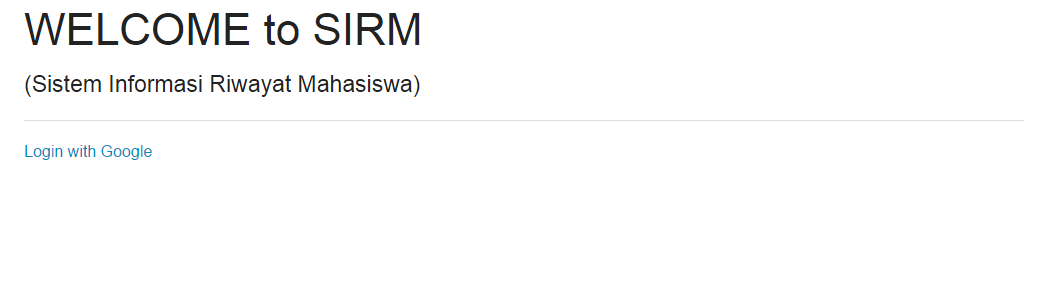
\includegraphics[scale=1]{Gambar/pengujian1.png}
\caption[Membuka Halaman index.php]{Membuka Halaman index.php} 
\label{fig:membukahalamanindex}
\end{figure}

\begin{figure}[H]
\centering
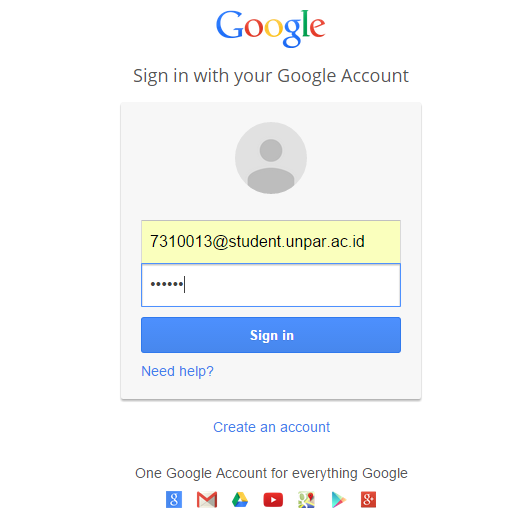
\includegraphics[scale=1]{Gambar/pengujian2.png}
\caption[Login Dengan Email yang Diakhiri "@student.unpar.ac.id"]{Login Dengan Email yang Diakhiri "@student.unpar.ac.id"} 
\label{fig:logindenganstudent}
\end{figure}

\begin{figure}[H]
\centering
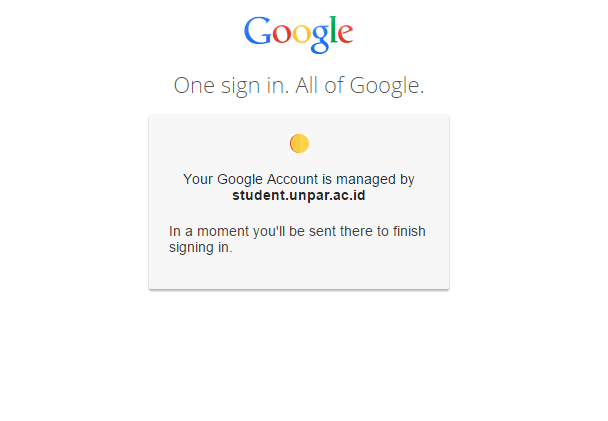
\includegraphics[scale=1]{Gambar/pengujian3.png}
\caption[Konfirmasi Email yang Dikelola oleh student.unpar.ac.id]{Konfirmasi Email yang Dikelola oleh student.unpar.ac.id} 
\label{fig:konfirmasiemail}
\end{figure}

\begin{figure}[H]
\centering
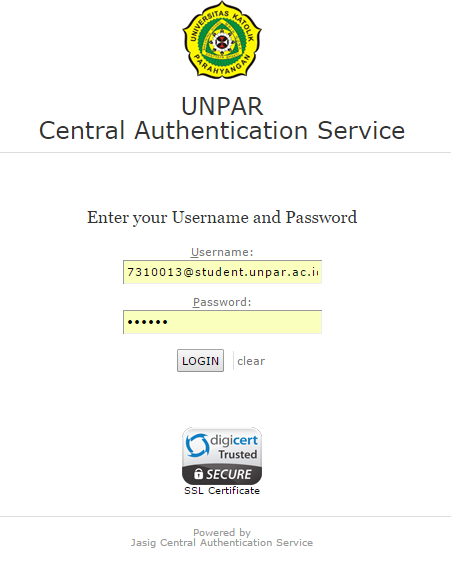
\includegraphics[scale=1]{Gambar/pengujian4.png}
\caption[CAS UNPAR]{CAS UNPAR} 
\label{fig:casunpar}
\end{figure}

\begin{figure}[H]
\centering
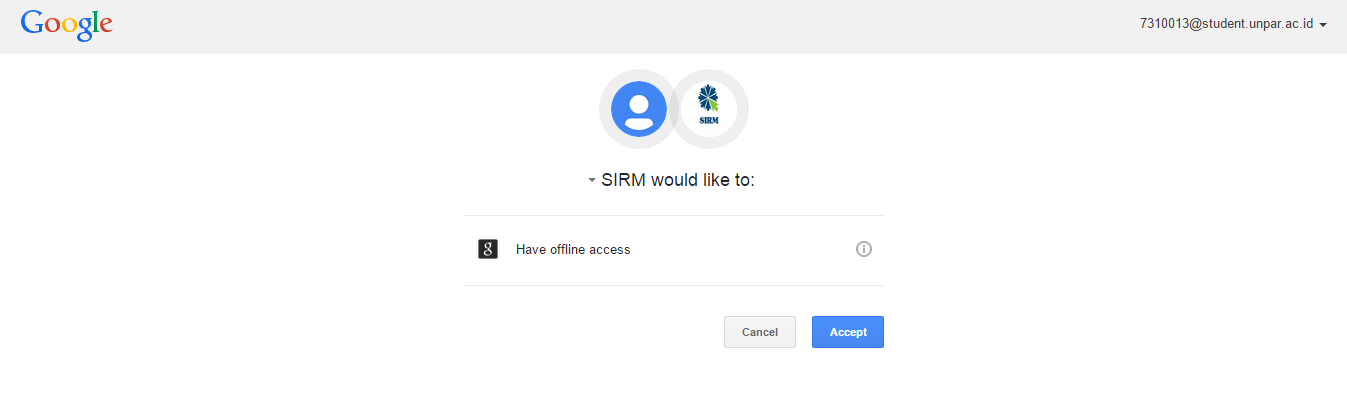
\includegraphics[scale=0.5]{Gambar/pengujian5.png}
\caption[Izin Akses Dari Pihak Pengguna]{Izin Akses Dari Pihak Pengguna} 
\label{fig:izindaripihakpengguna}
\end{figure}

\begin{figure}[H]
\centering
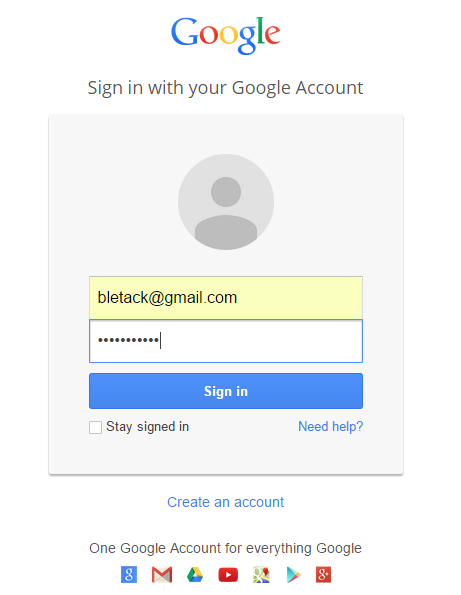
\includegraphics[scale=1]{Gambar/pengujian6.png}
\caption[Login Dengan Email yang Diakhiri "@gmail.com"]{Login Dengan Email yang Diakhiri "@gmail.com"} 
\label{fig:logindengangmail}
\end{figure}

\begin{figure}[H]
\centering
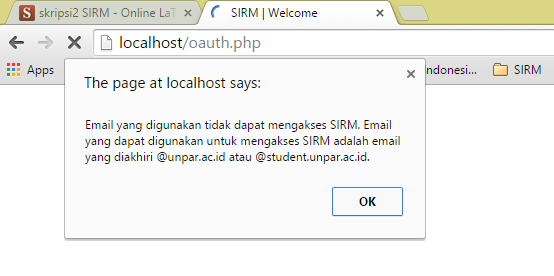
\includegraphics[scale=1]{Gambar/pengujian7.png}
\caption[Alert Email yang Digunakan Tidak Dapat Mengakses SIRM]{Alert Email yang Digunakan Tidak Dapat Mengakses SIRM} 
\label{fig:alert}
\end{figure}

\begin{figure}[H]
\centering
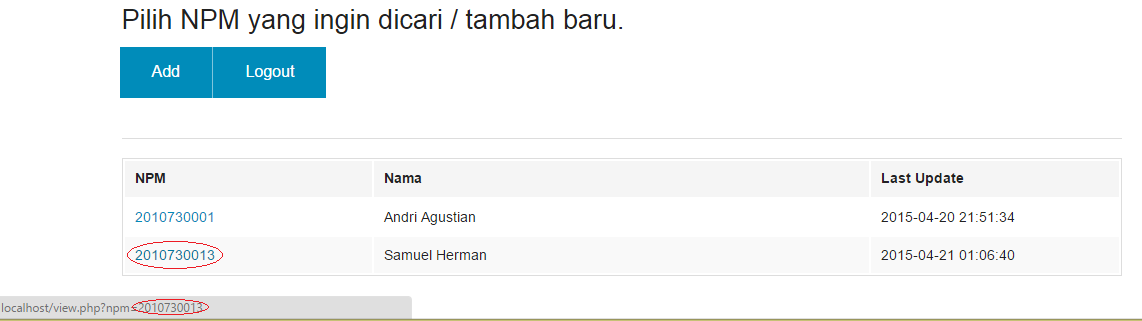
\includegraphics[scale=0.5]{Gambar/pengujian8.png}
\caption[Memilih Mahasiswa]{Memilih Mahasiswa} 
\label{fig:memilihmahasiswa}
\end{figure}

\begin{figure}[H]
\centering
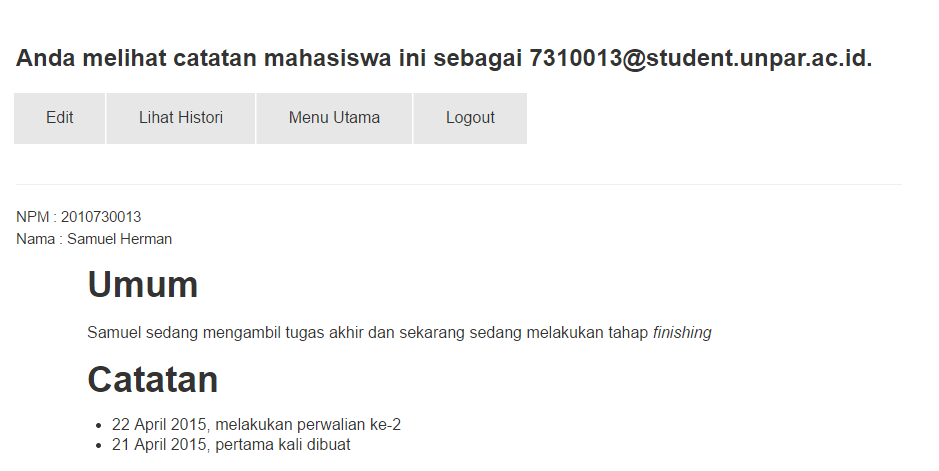
\includegraphics[scale=0.6]{Gambar/pengujian9.png}
\caption[Melihat Info Mahasiswa]{Melihat Info Mahasiswa} 
\label{fig:melihatinfomahasiswa}
\end{figure}

\begin{figure}[H]
\centering
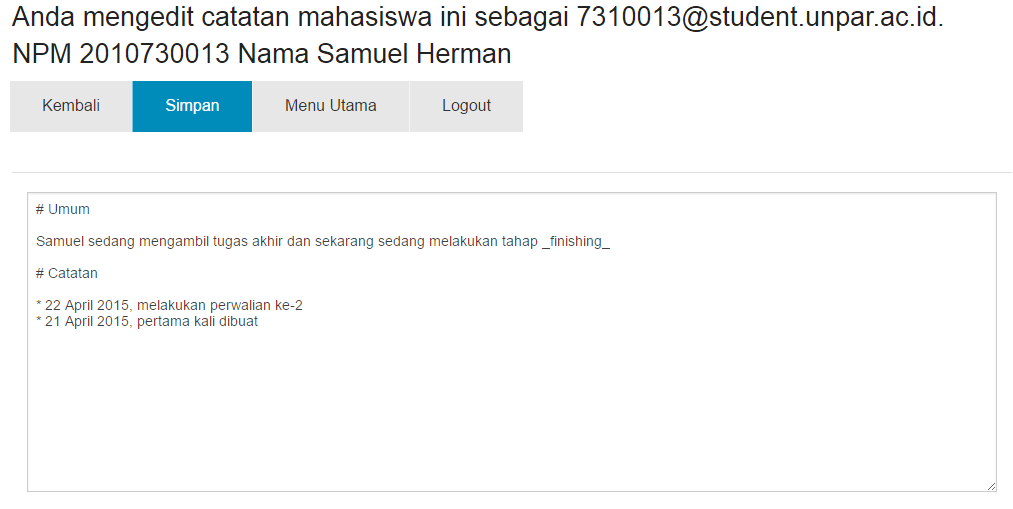
\includegraphics[scale=0.6]{Gambar/pengujian10.png}
\caption[Mengedit Info Mahasiswa]{Mengedit Info Mahasiswa} 
\label{fig:mengeditinfomahasiswa}
\end{figure}

\begin{figure}[H]
\centering
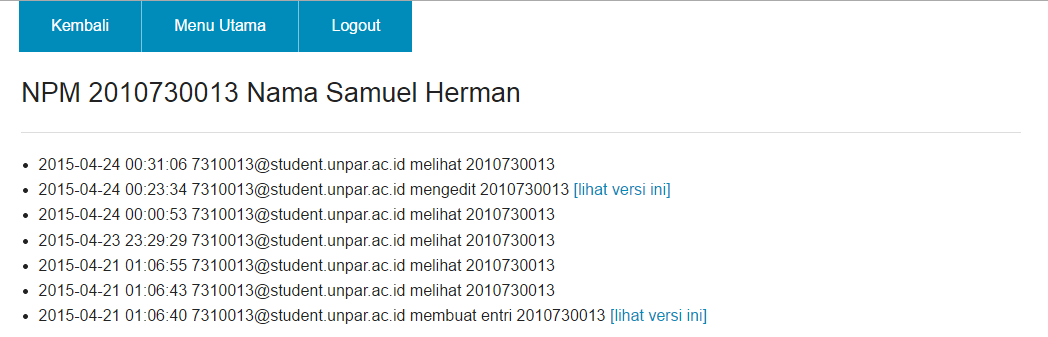
\includegraphics[scale=0.6]{Gambar/pengujian11.png}
\caption[Melihat Histori]{Melihat Histori} 
\label{fig:melihathistori}
\end{figure}

\begin{figure}[H]
\centering
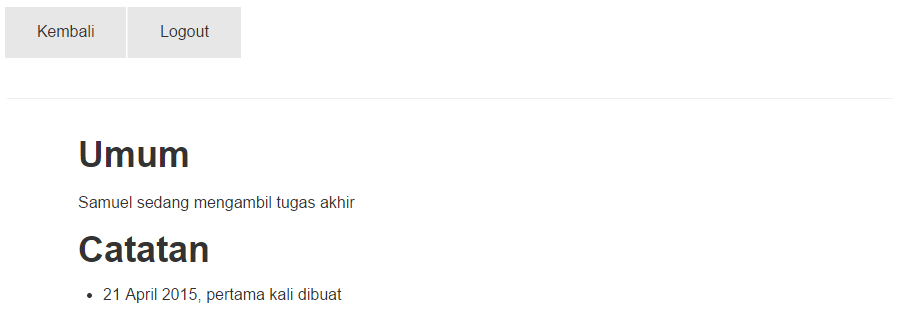
\includegraphics[scale=1]{Gambar/pengujian12.png}
\caption[Keterangan Versi Pertama]{Keterangan Versi Pertama} 
\label{fig:keteranganversipertama}
\end{figure}

\begin{figure}[H]
\centering
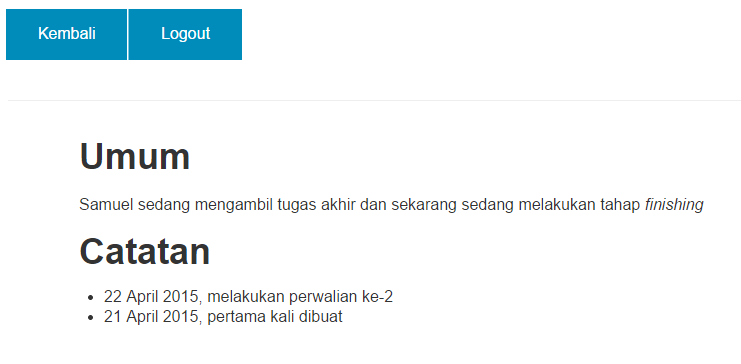
\includegraphics[scale=0.75]{Gambar/pengujian13.png}
\caption[Keterangan Versi Kedua]{Keterangan Versi Kedua} 
\label{fig:keteranganversikedua}
\end{figure}

\begin{figure}[H]
\centering
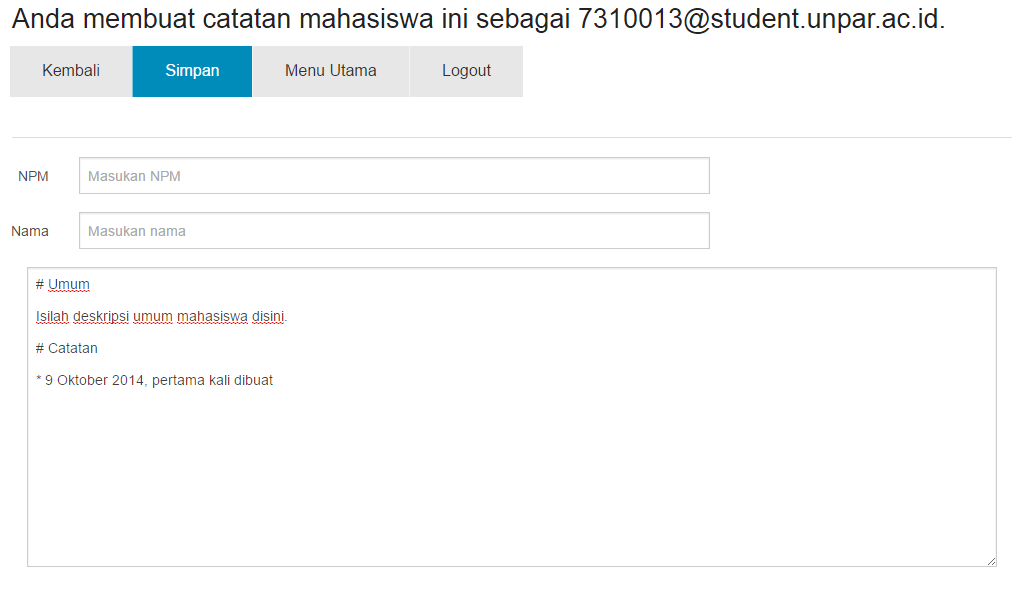
\includegraphics[scale=0.6]{Gambar/pengujian14.png}
\caption[Template Entri Baru]{Template Entri Baru} 
\label{fig:templateentribaru}
\end{figure}

\begin{figure}[H]
\centering
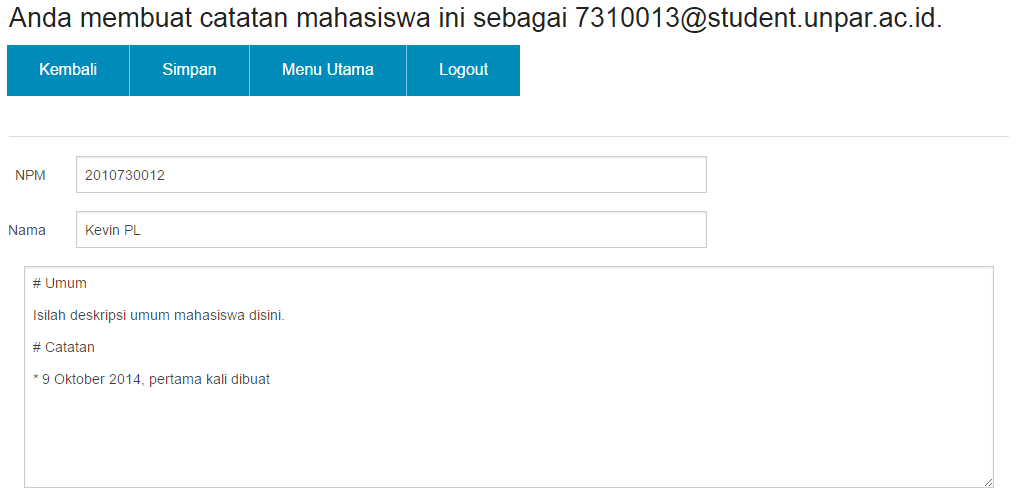
\includegraphics[scale=0.6]{Gambar/pengujian15.png}
\caption[Membuat Entri Baru]{Membuat Entri Baru} 
\label{fig:membuatentribaru}
\end{figure}

\begin{figure}[H]
\centering
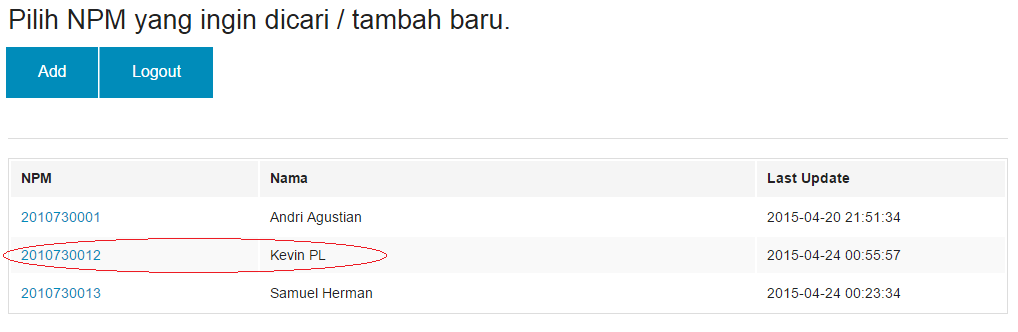
\includegraphics[scale=0.6]{Gambar/pengujian16.png}
\caption[Entri Baru Berhasil Dibuat]{Entri Baru Berhasil Dibuat} 
\label{fig:entribaruberhasil}
\end{figure}

\subsection{Hasil Pengujian Fungsional}
\label{sec:hasilpengujianfungsional}
Hasil pengujian fungsional dapat dilihat pada Tabel \ref{tab:hasilpengujianfungsional}.

\begin{center}
\begin{table}
\caption[Tabel 5-1 Hasil Pengujian Fungsional]{Hasil Pengujian Fungsional}\\
\label{tab:hasilpengujianfungsional}
\begin{center}
\begin{tabular}{|1|1|1|1|1|}
\hline
No & Aksi pengguna & Hasil yang diharapkan & Hasil yang didapatkan &
Keterangan\\
\hline
1 & \cmark & \cmark & \cmark & Berhasil\\
\hline
2 & \cmark & \cmark & \cmark & Berhasil\\
\hline
3 & \cmark & \cmark & \cmark & Berhasil\\
\hline
4 & \cmark & \cmark & \cmark & Berhasil\\
\hline
5 & \cmark & \cmark & \cmark & Berhasil\\
\hline
6 & \cmark & \cmark & \cmark & Berhasil\\
\hline
\end{tabular}
\end{center}
\end{table}
\end{center}

\subsection{Pengujian Eksperimental}
\label{sec:pengujianeksperimantal}
Pengujian eksperimental dilakukan kepada dua kelompok mahasiswa. Kelompok
pertama adalah mahasiswa jurusan teknik informatika dan kelompok kedua
adalah mahasiswa jurusan non-teknik informatika. Kepada semua penguji baik
kelompok pertama maupun kelompok kedua telah dijelaskan terlebih dahulu apa itu
SIRM (Sistem Informasi Riwayat Mahasiswa), fungsi-fungsi yang terdapat pada SIRM, dan
mekanisme yang dapat berlaku pada SIRM. Kemudian semua penguji diberikan tugas
seolah-olah mereka adalah dosen yang menjalankan seluruh fungsi yang dimiliki
SIRM (login, melihat daftar mahasiswa, melihat info mahasiswa, mengedit info
mahasiswa, melihat histori mahasiswa, dan membuat entri baru)dan memahami SIRM
secara keseluruhan. Setelah selesai melakukan pengujian, penguji akan diminta
untuk mengisi angket. Penulis akan mengukur waktu selama pengujian dan mencatat
berapa waktu yang dibutuhkan penguji untuk memahami dan menjalankan setiap fungsi dengan benar.

Kelompok pertama terdiri dari empat orang mahasiswa jurusan teknik informatika.
Keempat penguji berhasil menjalankan dan memahami SIRM dengan baik. Untuk
catatan waktu yang dimiliki oleh kelompok pertama dapat dilihat pada Tabel
\ref{tab:catatanwaktukelompokpertama}. Rata-rata waktu yang diperlukan
kelompok pertama untuk menjalankan setiap fungsi dapat dilihat di bawah ini.
\begin{enumerate}[1]
  \item Login\\
  $$105 + 52 + 93 + 127 / 4 = 377 / 4 = 94.25 detik$$
  \item Melihat Daftar Mahasiswa
  $$31 + 8 + 11 + 7 / 4 = 57 / 4 = 14.25 detik$$
  \item Melihat Info Mahasiswa
  $$24 + 12 + 6 + 19 / 4 = 61 / 4 = 15.25 detik$$
  \item Mengedit Info Mahasiswa
  $$37 + 43 + 39 + 25 / 4 = 144 / 4 = 36 detik$$
  \item Melihat Histori Mahasiswa
  $$10 + 5 + 14 + 36 / 4 = 64 / 4 = 16.25 detik$$
  \item Membuat Entri Baru
  $$186 + 42 + 103 + 86 / 4 = 417 / 4 = 104.25 detik$$
\end{enumerate}

\begin{center}
\begin{table}
\caption[Tabel 5-2 Catatan Waktu Pengujian Eksperimental Kelompok
Pertama]{Catatan Waktu Pengujian Eksperimental Kelompok Pertama}\\
\label{tab:catatanwaktukelompokpertama}
\begin{center}
\begin{tabular}{|p{3cm}|p{1.5cm}|p{1.5cm}|p{1.5cm}|p{1.5cm}|}
\hline
Aksi & Penguji 1 & Penguji 2 & Penguji 3 & Penguji 4\\
\hline
Login & 1 menit 45 detik & 52 detik & 1 menit 33 detik & 2 menit 7 detik\\
\hline
Melihat Daftar Mahasiswa & 31 detik & 8 detik & 11 detik & 7 detik\\
\hline
Melihat Info Mahasiswa & 24 detik & 12 detik & 6 detik & 19 detik\\
\hline
Mengedit Info Mahasiswa & 37 detik & 43 detik & 39 detik & 25 detik\\
\hline
Melihat Histori Mahasiswa & 10 detik & 5 detik & 14 detik & 36 detik\\
\hline
Membuat Entri Baru & 3 menit 6 detik & 42 detik & 1 menit 43 detik & 1 menit
26 detik\\
\hline
\end{tabular}
\end{center}
\end{table}
\end{center}

Kelompok kedua terdiri dari empat orang mahasiswa jurusan non-teknik
informatika. Keempat penguji berhasil menjalankan dan memahami SIRM dengan baik.
Untuk catatan waktu yang dimiliki oleh kelompok kedua dapat dilihat pada Tabel
\ref{tab:catatanwaktukelompokkedua}. Rata-rata waktu yang diperlukan
kelompok kedua untuk menjalankan setiap fungsi dapat dilihat di bawah ini.
\begin{enumerate}[1]
  \item Login\\
  $$168 + 117 + 99 + 129 / 4 = 513 / 4 = 128.25 detik$$
  \item Melihat Daftar Mahasiswa
  $$66 + 63 + 68 + 58 / 4 = 255 / 4 = 63.75 detik$$
  \item Melihat Info Mahasiswa
  $$67 + 63 + 46 + 2 / 4 = 178 / 4 = 44.5 detik$$
  \item Mengedit Info Mahasiswa
  $$64 + 90 + 73 + 48 / 4 = 275 / 4 = 68.75 detik$$
  \item Melihat Histori Mahasiswa
  $$72 + 66 + 94 + 67 / 4 = 299 / 4 = 74.75 detik$$
  \item Membuat Entri Baru
  $$68 + 138 + 124 + 205 / 4 = 535 / 4 = 133.75 detik$$
\end{enumerate}

\begin{center}
\begin{table}
\caption[Tabel 5-3 Catatan Waktu Pengujian Eksperimental Kelompok
Kedua]{Catatan Waktu Pengujian Eksperimental Kelompok kedua}\\
\label{tab:catatanwaktukelompokkedua}
\begin{center}
\begin{tabular}{|p{3cm}|p{1.5cm}|p{1.5cm}|p{1.5cm}|p{1.5cm}|}
\hline
Aksi & Penguji 1 & Penguji 2 & Penguji 3 & Penguji 4\\
\hline
Login & 2 menit 48 detik & 1 menit 57 detik & 1 menit 39 detik & 2 menit 9
detik\\
\hline
Melihat Daftar Mahasiswa & 1 menit 6 detik & 1 menit 3 detik & 1 menit 8 detik &
58 detik\\
\hline
Melihat Info Mahasiswa & 1 menit 7 detik & 1 menit 3 detik & 46 detik & 2
detik\\
\hline
Mengedit Info Mahasiswa & 1 menit 4 detik & 1 menit 30 detik & 1 menit 13 detik
& 48 detik\\
\hline
Melihat Histori Mahasiswa & 1 menit 12 detik & 1 menit 6 detik & 1 menit 34
detik & 1 menit 7 detik\\
\hline
Membuat Entri Baru & 1 menit 8 detik & 2 menit 18 detik & 2 menit 4 detik & 3
menit 25 detik\\
\hline
\end{tabular}
\end{center}
\end{table}
\end{center}

Perbandingan dari rata-rata waktu pengujian eksperimental antara kelompok
pertama dan kelompok kedua dapat dilihat pada Tabel
\ref{tab:perbandinganrataratawaktu}.

\begin{center}
\begin{table}
\caption[Tabel 5-4 Perbandingan Rata-rata Waktu Pengujian Eksperimental]{Perbandingan Rata-rata Waktu Pengujian Eksperimental}\\
\label{tab:perbandinganrataratawaktu}
\begin{center}
\begin{tabular}{|p{3cm}|1|1|p{3cm}|}
\hline
Aksi & Kelompok Pertama & Kelompok Kedua & Keterangan\\
\hline
Login & 94.25 detik & 128.25 detik & Kelompok pertama lebih cepat 34 detik
dari kelompok kedua\\
\hline
Melihat Daftar Mahasiswa & 14.25 detik & 63.75 detik & Kelompok pertama lebih
cepat 49.5 detik dari kelompok kedua\\
\hline
Melihat Info Mahasiswa & 15.25 detik & 44.5 detik & Kelompok pertama lebih cepat
29.25 detik dari kelompok kedua\\
\hline
Mengedit Info Mahasiswa & 36 detik & 68.75 detik & Kelompok pertama lebih cepat
32.75 detik dari kelompok kedua\\
\hline
Melihat Histori Mahasiswa & 16.25 detik & 74.75 detik & Kelompok pertama lebih
cepat 58.5 detik dari kelompok kedua\\
\hline
Membuat Entri Baru & 104.25 detik & 133.75 detik & Kelompok pertama lebih cepat
29.5 detik dari kelompok kedua\\
\hline
\end{tabular}
\end{center}
\end{table}
\end{center}

